% !TEX root = main.tex

%%%%%%%%%%%%%%%%%%%%%%%%%%%%%%%%%%%%%%%%%%%%%%%%%%%%%%%%%%%%%%%%%%%%%%%%%%%%%%%%
\chapter{Introduction}

The 3D scanning of outdoor structures has gained a lot of interest recently. The emergence of cheap and easy-to-use 3D sensors brought its share of new applications, enabling the digitization of the world by the masses. Most of common everyday 3D scanning devices are captive of the indoors, though. There is yet to find a way to give everyone the chance to scan building-scale objects, bridging the gap between indoor and outdoor scanning. Stereo triangulation techniques such as Structure from Motion certainly answers some of these needs, but won't give high-detail reconstructions, especially on textureless surfaces.

This thesis proposes to do so simply by using cameras, and an existing reconstruction technique dubbed ``Photometric Stereo'' (PS). The idea is to point a camera towards a scene to be scanned, and to capture a time-lapse sequence. Variations in the illumination conditions can be used by PS to reconstruct the shape of the observed scene. PS has been known in computer vision for more than 35 years, and is still an active area of research, but outdoor performance is far from matching performance in laboratory conditions because of the uncontrolled natural illumination. It is an excellent choice for shape reconstruction given its great output density and stellar results in laboratory conditions.

\section{Photometric Stereo}
\label{sec:ps_ori}

The first definition of PS, made in 1979 by Woodham~\cite{Woodham1979}, made a lot of assumptions to simplify the problem to its essence. For example, the surface reflectance must be Lambertian, meaning that light is reflected equally in all directions, and constant over the whole image and over time. The object should also be rigid, meaning that the surface should not move through time. The lighting must be known a priori and consist of of a distant point light source. All the images are supposed perfectly aligned through time, meaning that both the camera and the target are static. In its essence, everything must be constant; only the illumination should vary over the sequence, and, as a result, pixel intensity varies with the illumination. Even today, most of these assumptions are still found in state-of-the-art outdoor PS, which remains a difficult problem that has received considerably less attention compared to PS in the lab. 

Under the Lambertian assumption, each image pixel $p$ depicts a surface patch with albedo $\rho_p$ and normal $n_p$. Under the illumination of a distant point light (directional) source, $\mathbf{l}_t^T \in \mathbb{R}^3$ at time $t$, the observed pixel intensity $b_p$ follows the Lambertian image formation model:
\begin{equation}
b_t =  \rho \; \mathbf{l}^T \mathbf{n}_p \quad.
\end{equation}
For the sake of simplification, the incident lighting vector $\mathbf{l}$ is scaled by its intensity.

This means that the appearance of a pixel in an image, with the aforementioned assumptions, is dependent on 1) the normal and albedo of a visible surface patch, and 2) the incident angle and intensity of the light. Woodham realized that if a pixel appearance depends on the surface normal, it meant that this surface normal can be found from a known pixel appearance. Because the normals are related to surface gradients, which can be integrated to recover a detailed surface, this means that the shape of an object (through its surface normals) could be obtained by observing the pixels appearance. But there's a problem: a single image of a surface patch (a pixel) cannot explain all three degrees of freedom of the normal to be reconstructed (scaled by its albedo), leading to an underconstrained problem known as shape from shading (SfS)~\cite{Horn1989}.

To solve this issue, PS considers as input a sequence of images, all from the same viewpoint, but with different lighting conditions ${\bf l}_t$. The shading difference between the different lighting conditions can constrain the problem correctly. An example of such image sequence is shown in fig.~\ref{fig:PS_example}. In the case of a sequence of images, we define $\mathbf{L}$ as the stacked incident vectors of all the $m$ images in the sequence (labeled $\mathbf{l}_{1}, \mathbf{l}_{2}, \dots \mathbf{l}_{m}$):
\begin{equation}
\mathbf{L} \in \mathbb{R}^{m \times 3} =
\begin{bmatrix}
    \mathbf{l}_{1}^T \\
    \mathbf{l}_{2}^T \\
    \vdots \\
    \mathbf{l}_{m}^T
\end{bmatrix}
\quad,
\end{equation}
which can be used to define the appearance of all pixels over all the images of the sequence, as such:
\begin{equation}
\label{eq:lamb_refl}
\mathbf{b} =  \rho \mathbf{L} \mathbf{n}_p \quad,
\end{equation}
for ${\bf b} \in \mathbb{R}^{m \times k}$ for images of $k$ pixels. This definition needs the pixels intensities from the image sequence to be vectorized, meaning that every image must be reshaped to be $\mathbb{R}^{1 \times k}$

Solving eq.~\eqref{eq:lamb_refl} for a particular surface patch $\mathbf{n}$ (corresponding pixel coordinates in all images) gives the relation
\begin{equation}
\label{eq:original_form}
\rho \mathbf{n}_p =  \mathbf{L}^{-1} \mathbf{b} \quad,
\end{equation}
giving birth to the Photometric Stereo technique.

The normal $\mathbf{n}$ provides the structure of the scene visible in the image sequence, giving a single normal for each pixel of the image, as shown in fig.~\ref{fig:PS_example_res}. This output is called a normal map, because it maps a surface normal to each surface patch visible by a pixel. Integrating this normal map results in an height map (also called depth map), which represents the height of the surface at each sample point. To summarize, PS outputs a normal map, the gradient of the height map.

The great strength of this technique is its output density: 3D information will be generated for every pixel of one input image. This means that a sequence of 5 megapixels images, as can be found on many current off-the-shelf cameras and cellphones, will generate an output of 5 million 3D points using PS. This quantity of information is impressive given the cost of point and shoot cameras and the ubiquity of cellphones.

Dense stereo matching techniques also provides a depth per pixel, rivaling with PS in terms of information density. But to work, these techniques requires regularization, which smooths the surface, whereas PS directly recovers normals (surface gradients), providing surface detail.

In order to work, PS requires the lighting directions to be known (either by controlling the illumination in the laboratory~\cite{Woodham1979,Ikeuchi1981} or capturing a mirror sphere~\cite{inose-tcva-13,hung-wacv-15,ikehata-cvpr-14,oxholm-eccv-12,ikehata-cvpr-12,Ackermann2012a,Lu2012,shi-cvpr-10,yu-iccp-13,shi-3dv-14}) Even with all the assumption we made, one issue remains: the lighting directions over the sequence must not be coplanar. If they are coplanar, $\mathbf{L}$ is rank-2 and singular, meaning the $\mathbf{L}^{-1}$ does not exist in eq.~\ref{eq:original_form}. This led Woodham to believe that PS ``does not apply to outdoor images taken at different times during the same day [...] since the sun's path across the sky is planar''~\cite{Woodham1979}.

%\begin{equation}
%\mathbf{b} = \rho L(\mathbf{\boldomega}) \langle \boldomega, {\bf n} \rangle \,,
%\end{equation}

\begin{figure}
\centering
%\begin{tabular}{cccccc|ccc}

\includegraphics[width=.15\linewidth]{PS/cat_0.png}

\includegraphics[width=.15\linewidth]{PS/cat_3.png}

\includegraphics[width=.15\linewidth]{PS/cat_4.png}

\includegraphics[width=.15\linewidth]{PS/cat_5.png}

\includegraphics[width=.15\linewidth]{PS/cat_10.png}

\includegraphics[width=.15\linewidth]{PS/cat_11.png}
%
\includegraphics[width=.08\linewidth]{PS/cat_normal_map.png}
%
\includegraphics[width=.04\linewidth]{PS/sphere_nm.png}
%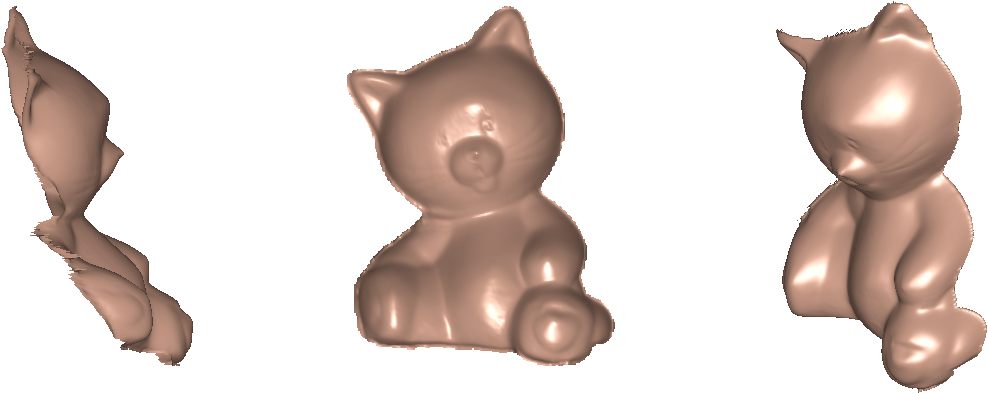
\includegraphics[width=.18\linewidth]{PS/3d.png}
%a) & b) & c) & d) & e) & f) & g) & h) & i)
%\end{tabular}
\caption{Examples of inputs lit from different directions, g) normal map obtained from the original form of the Photometric Stereo algorithm, h) sphere normal map showed as example, i) reconstructed surface from 3 viewpoints.\newline
{\small input images from CSE 455, 2010 by Neel Joshi, Ira Kemelmacher and Ian Simon}
}
\label{fig:PS_example}
\end{figure}

\begin{figure}
\begin{tabular}{ccc}

\includegraphics[height=3.8cm]{PS/cat_normal_map.png} &

\includegraphics[width=.15\linewidth]{PS/sphere_nm.png} &
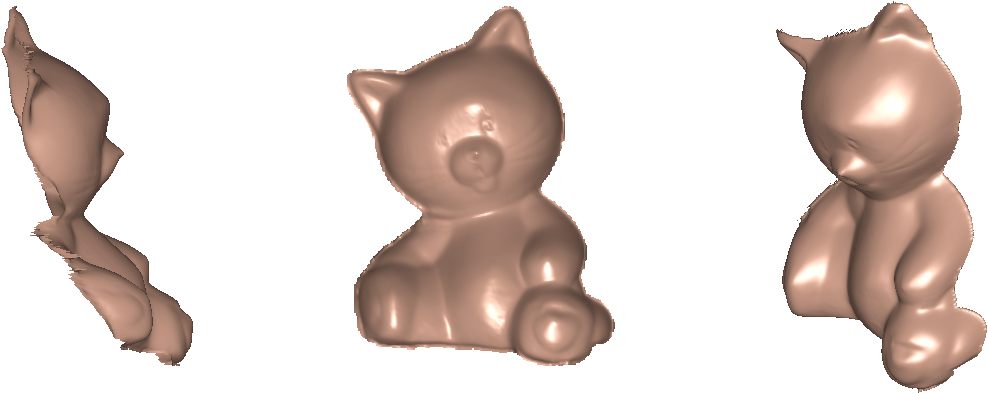
\includegraphics[height=3.8cm]{PS/3d.png} \\
(a) & (b) & (c)
\end{tabular}
\caption{Results from the inputs in \ref{fig:PS_example}. (a) normal map obtained from the original form of the Photometric Stereo algorithm, (b)) sphere normal map showed as example, (c)) reconstructed surface from 3 viewpoints.}
\label{fig:PS_example_res}
\end{figure}

\section{Outdoor Photometric Stereo}

A lot of work have been done on PS since its original definition. Contrary to what Woodham believed, PS has recently been applied to outdoor photographs, mainly images captures by outdoor cameras. Unfortunately, outdoor lighting is complex and uncontrollable. Over the course of a day, the sun trajectory lies on a single plane, giving coplanar lighting directions, leading to a singular lighting matrix $\mathbf{L}$. A technique proposed to circumvent this issue is to capture many months of data. This will allow the sun trajectory to shift enough to condition correctly the PS formulation. This idea works, but is not a very practical scenario for the casual user.

\begin{figure}
\centering
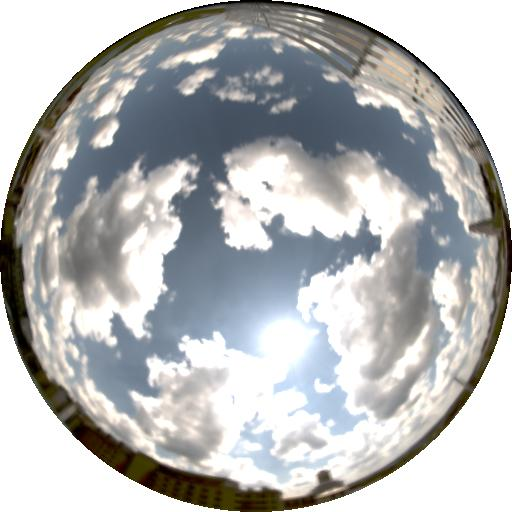
\includegraphics[width=0.5\linewidth]{./figures/database/20130824_140002.jpg}
\caption{Example environment map shown using the Sky Angular projection. On this projection, the horizon is located on the circumference of the image and the zenith (up) is located in the center.}
\label{fig:envmap_example}
\end{figure}


To make PS work outdoor, the traditionally employed approximation models such as directional lighting will be replaced by a new data-driven model of natural illumination learned from a large database of high quality sky photographs. This database was (and will be) captured over extended periods of time, and already contain thousands of photos of the sky in different illumination conditions. By observing the sky directly, the data-driven model will accurately capture what the likely natural illumination conditions are for a given scene. An example of such photograph is shown in fig.~\ref{fig:envmap_example}. From this capture, we can get a glimpse of the complexity of outdoor illumination. Notice how this image is not composed only of a sun, but contains a sky scattering the sunlight in the atmospheres, clouds that may occlude the sun, an so forth. An enhanced lighting model taking into account all these phenomenons will better constrain the PS optimization algorithm, allowing it to converge toward real or plausible sky illumination conditions. The resulting shape estimation will better explain the observed input images, giving increased result quality. People already shown that exploring more complex illumination models is advantageous in PS, but a lot of questions remain. To goal of my work is to answer as many of these questions as possible.


\section{Thesis proposal}

The main goal of this thesis is to \textbf{understand how natural illumination impacts PS, effectively tying the reconstruction performance to the sky appearance}. This leads to multiple applications, such as large-scale outdoor scenes reconstruction from short time intervals.

In this thesis, I propose to:
\begin{enumerate}
  \item bring a deeper understanding of the way PS can work outdoors;
  \item introduce a practical PS reconstruction algorithm in the calibrated case, where the lighting conditions are known;
  \item introduce a practical PS reconstruction algorithm in the uncalibrated case, where the lighting conditions are unknown;
\end{enumerate}
These objectives can be attained by a better comprehension of natural illumination and its impact on shading. This knowledge can then be leveraged to improve existing reconstruction algorithms or design new ones that works with complex and uncontrolled lighting conditions.

This thesis will bring answers to questions like:
\begin{itemize}
  \item What is the minimum timelapse interval required to perform PS outside? (e.g.\ a whole day? $x$ hours?)
  \item What sky characteristics are tied to PS reconstruction performance? Are cloudy, sunny, or both days the best for PS?
  \item How can we reconstruct an object with natural illumination using PS?
  \item Can the moon be used as a light source during the night to perform PS during the night? What performance enhancement can I expect from a 24 hours capture (day and night)?
\end{itemize}

\section{Anticipated impact}

3D scanning has become a part of everyday life, with sensors such as the Kinect now in everyone's home, effectively bringing 3D scanning capabilities to the masses. Taking the Kinect as example, a plethora of new use cases emerged since its original endeavor to revitalize the entertainment industry. For instance, the 3D printing market that grew significantly over the past few years, brought a new need for scans of household objects. Augmented reality is another avenue that requires a lot of models of real world objects. These are but a tiny fraction of the applications of real world scanning.

While the Kinect enabled myriads of applications in indoor environments, using such sensors outdoors is close to impossible. These kind of sensors are so-called active sensors, meaning that they interact with the scene to work. This usually means projecting light in the scene and sensing it back. But this method is problematic outside: the light patterns they emit are completely drowned by the sunlight. In outdoor settings, the only current possibilities are either to use very expensive scanners, out of reach for the casual user due to their complexity and operational cost, or structure from motion, giving a low level of detail or failing on textureless surfaces. The idea is to bring back the availability and cheapness of sensors such as the Kinect to the outside world, while obtaining a high level of detail on the reconstructed objects.

The level of understanding I propose in this thesis would allow the design and implementation a 3D shape acquisition system that relies only on off-the-shelf cameras, capable of bringing high quality digitization capabilities to anyone with a camera, thus enabling the collaborative reconstruction of large scale outdoor environments. This has the potential of impacting many fields, such as the high-detail digital preservation of cultural heritage before it gets damaged by wars, natural disasters, or the passage of time; the replication of real environments in virtual scenarios for the training of first responders or to improve urban planning; the creation of novel, realistic environments for use in video games or special effects in the movie industry; etc. By making these tasks easier, I believe this project will have significant impact on 3D shape acquisition as a whole.